%===================================== CHAP 5 =================================

\chapter{Implementation}

\figurename~\ref{fig:architecture-overview} shows a high level overview of the
CARP hardware platform extended with a readout module. While the system has been
extended with new functionality and partially ported to Chisel, the overall
architecture of the system has been largely preserved. In
\figurename~\ref{fig:architecture-detail}, a more detailed view of the system is
shown. Modules are annotated with either a C(hisel) or a V(HDL) in the upper
right corner to indicate their porting status. The top level logic and wiring
gluing all the modules together is all done in Chisel.

\begin{figure}[ht]
  \centering
  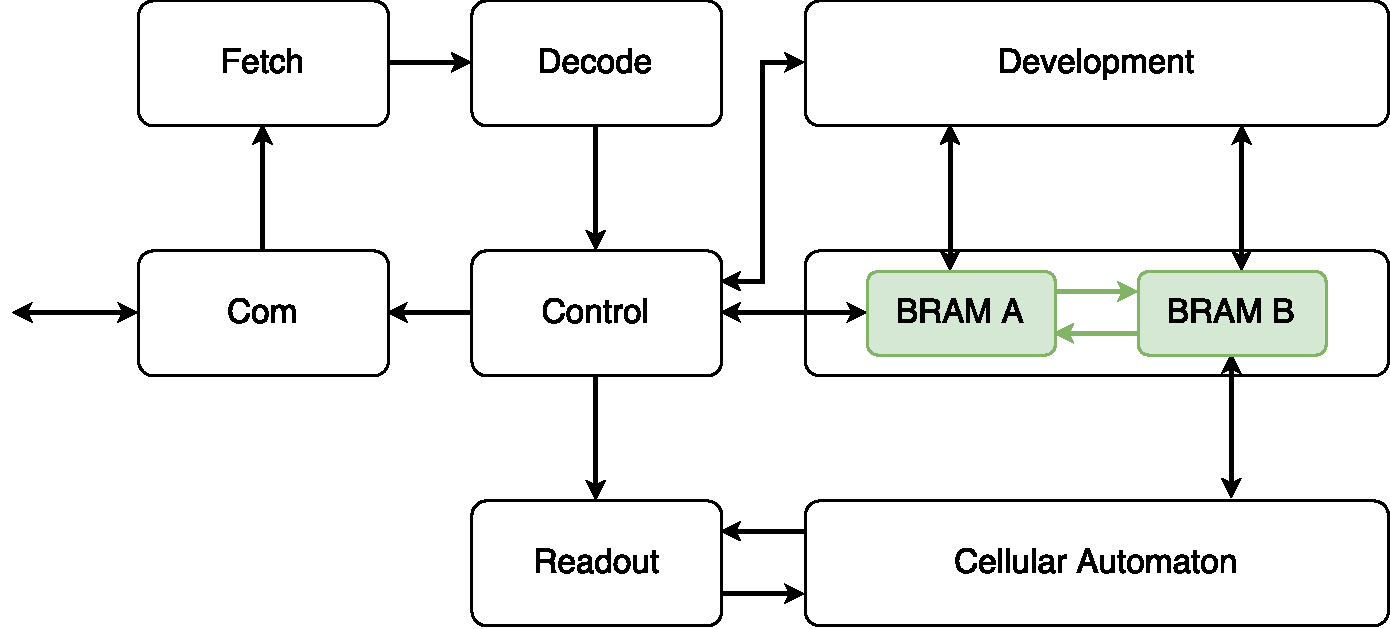
\includegraphics[width=0.8\linewidth]{fig/architecture-overview}
  \caption{
    Block diagram of the CARP hardware architecture extended with a readout layer.
  }
  \label{fig:architecture-overview}
\end{figure}

\begin{sidewaysfigure}[ht]
    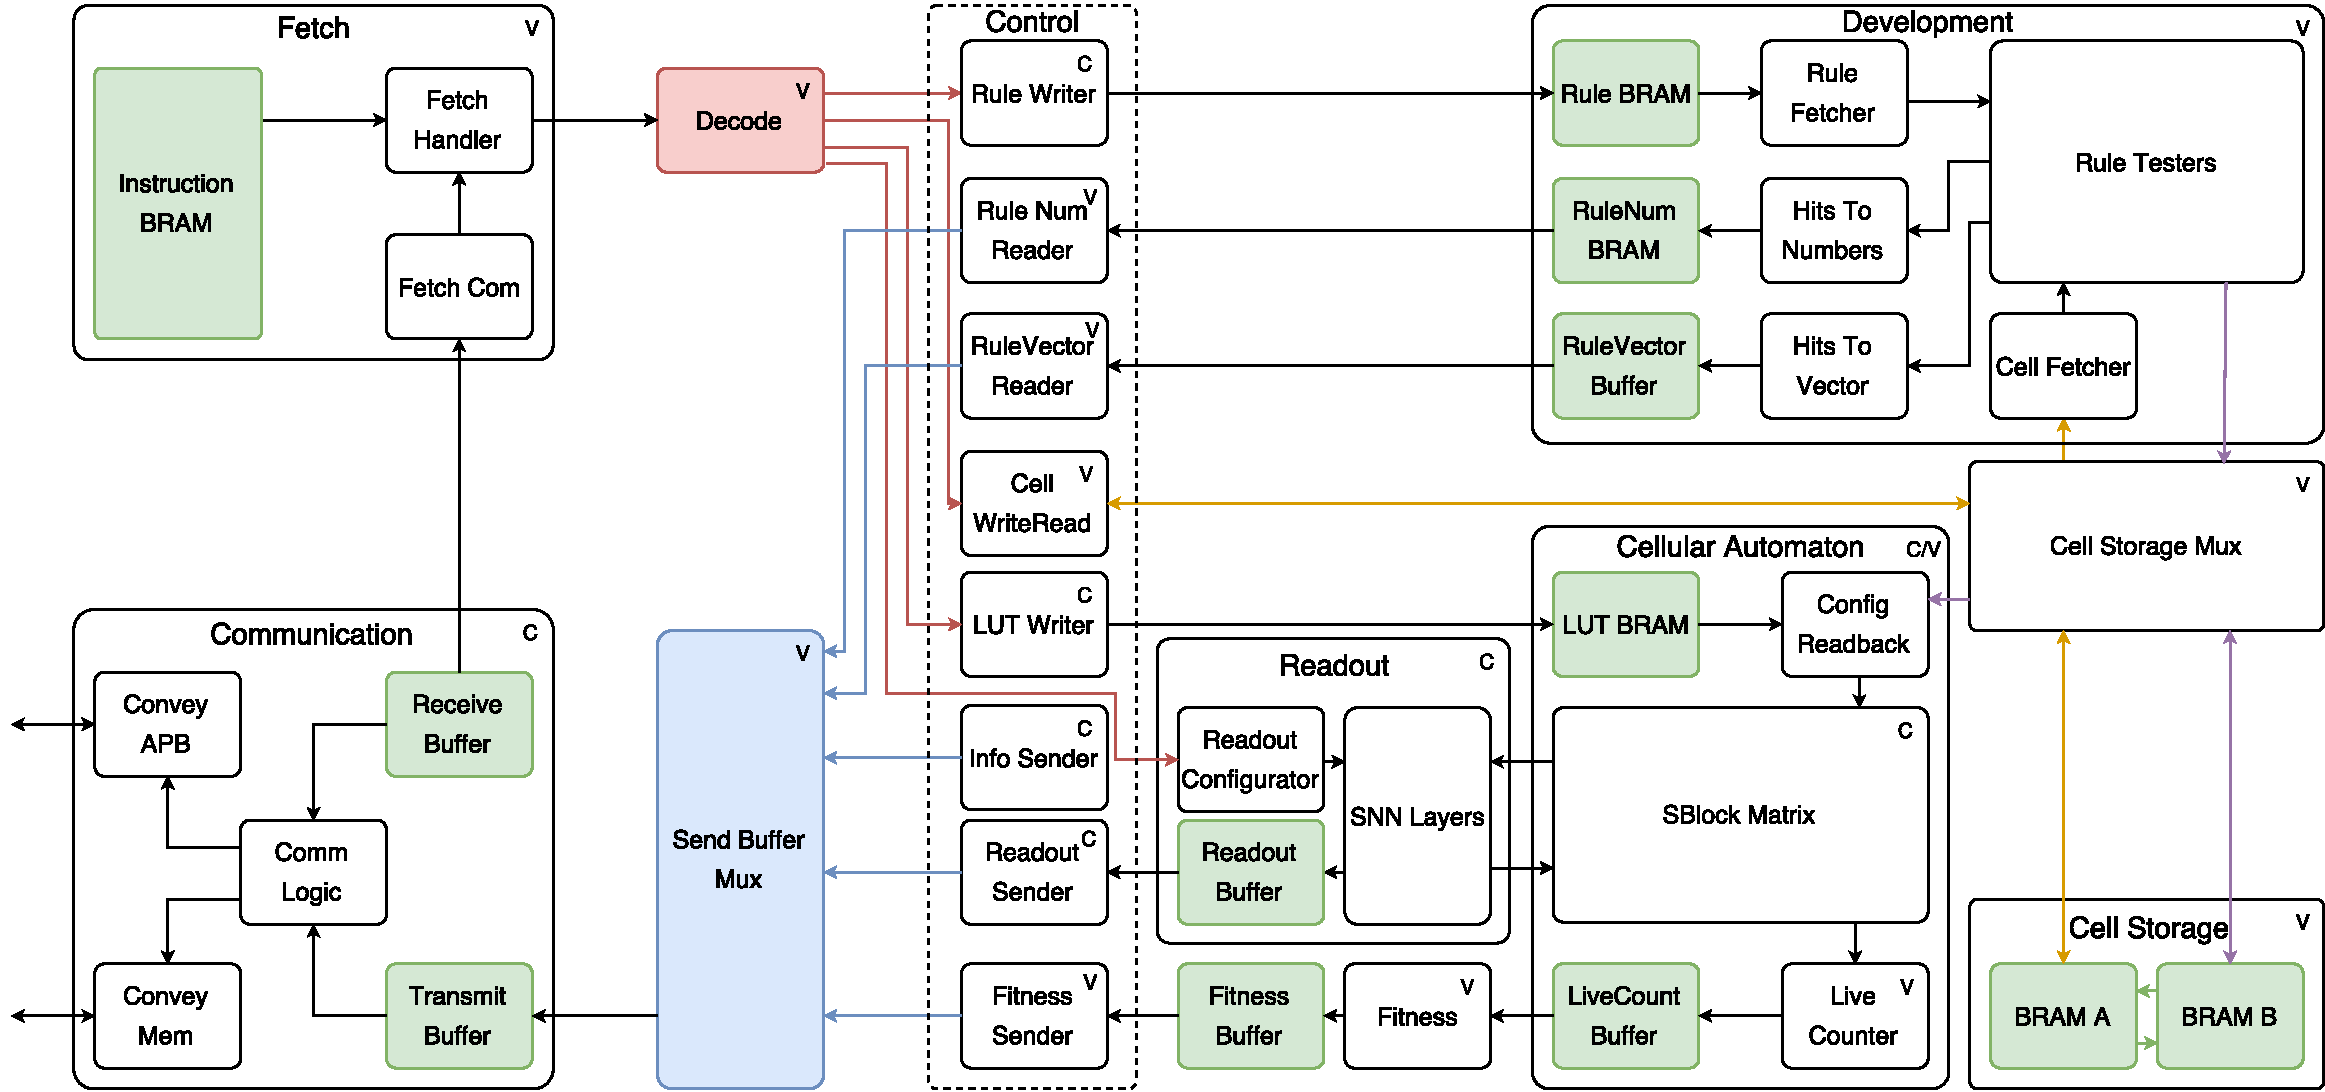
\includegraphics[width=\textwidth]{fig/architecture-detail}
    \caption{
      Modified reprint from~\cite{Lundal2015a} showing a detailed overview of
      the CARP architecture and its constituent modules. Modules annotated with a C in
      the upper right corner are implemented in / have been ported to Chisel, while
      those annotated with a V are implemented in VHDL. Child modules not annotated
      are implemented in the same language as their parent modules. Signals indicate
      flow of data or direction of communication, control signals and detailed
      interfaces are ommited for clarity.
    }
    \label{fig:architecture-detail}
\end{sidewaysfigure}
\clearpage

\section{General overview}

This section gives an overview of the modules involved in each of the three
pipeline stages

\subsection{Fetch}

\subsection{Decode}

\subsection{Execute}

\clearpage

\section{Communication}

As outlined in section~\ref{sec:coproc}, the FPGA on the Convey coprocessor is
logically divided into Application Engines within which any custom logic can be
implemented. Each AE can communicate with the host, the on-board memory and
other AEs through various interfaces implemented by the Convey PDK, shown in
\figurename~\ref{fig:convey-ae-io-overview}. To be able to run the CARP hardware
platform on the coprocessor, the communication module has been reimplemented to
utilize these interfaces for data transfer.

\begin{figure}[ht]
  \centering
  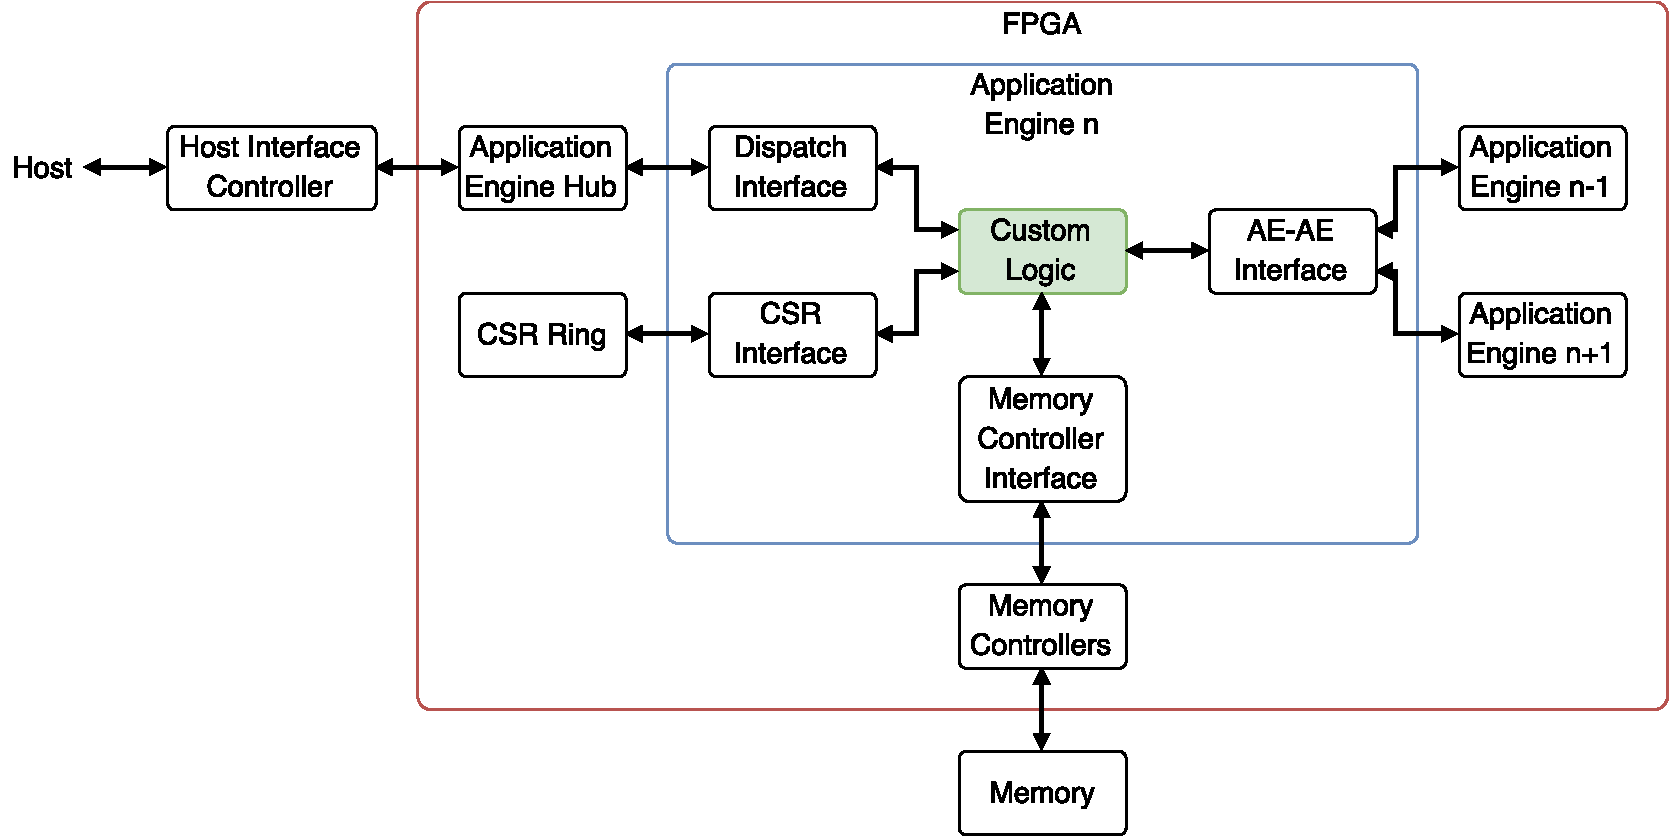
\includegraphics[width=\linewidth]{fig/convey-ae-io-overview}
  \caption{Overview of the Convey Application Engine architecture.}
  \label{fig:convey-ae-io-overview}
\end{figure}

\figurename~\ref{fig:convey-io-carp-overivew} shows how the CARP hardware is
implemented within the Convey AE architecture. The communication module has been
moved out of the main CARP module and rewritten from scratch. In an effort to
decouple the CARP platform from the underlying hardware and its communication
interfaces, the new module exposes two very generic interfaces facing
``outward,'' an Advanced Peripheral Bus (APB)
\footnote{\url{http://infocenter.arm.com/help/index.jsp?topic=/com.arm.doc.ihi0024c/index.html}
(Requires registration)} and a memory bus, as shown in
\figurename~\ref{fig:comm-io}. These are specified fully in
Appendix~\ref{app:interfaces}. Using generic interfaces with established
conventions that are easy to connect to other communication interfaces makes it
easy to move the system to a different platform, should the Convey coprocessors
become obsolete or defunct.

\begin{figure}[ht]
  \centering
  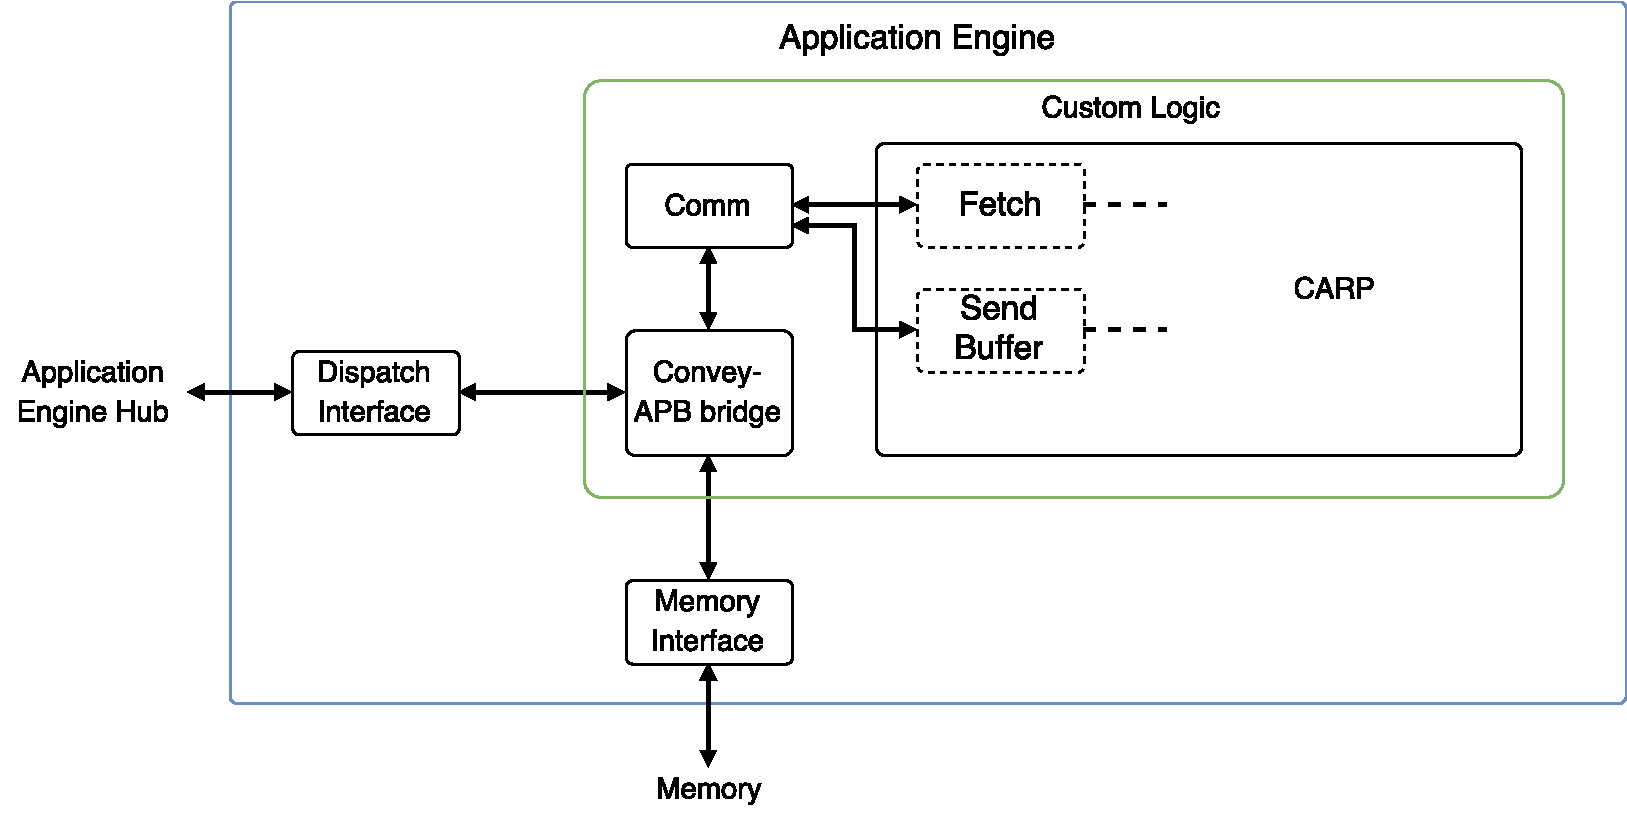
\includegraphics[width=\linewidth]{fig/convey-io-carp-overview}
  \caption{Implementation of the CARP platform within the AE architecture.}
  \label{fig:convey-io-carp-overivew}
\end{figure}

\begin{figure}[ht]
  \centering
  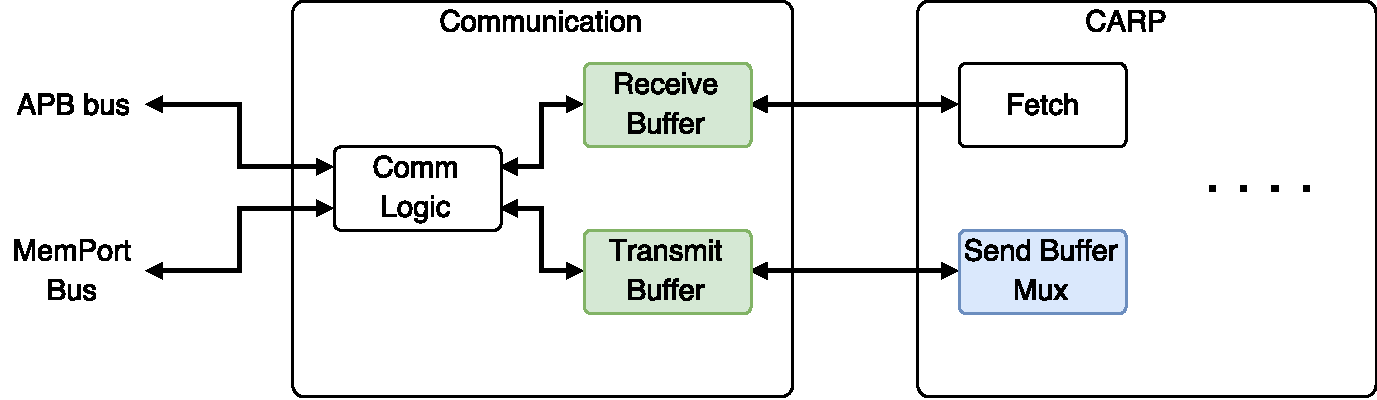
\includegraphics[width=0.8\linewidth]{fig/comm-io}
  \caption{
    The communication module interfaces with the CARP platform through two
    buffers, transmit and receive. Outwards, the communication module exposes two
    buses, an APB bus and a generic memory interface.
  }
  \label{fig:comm-io}
\end{figure}

To avoid having to rewrite the Fetch and Send Buffer Mux modules inside CARP,
the new communication module provides the same interface towards them as the old
one did; two data buffers, transmit and receive, buffer count signals and
read/write enable signals. Both data buffers are implemented as FIFO-queues with
counter registers and ready-valid access interfaces.

\begin{figure}[ht]
  \centering
  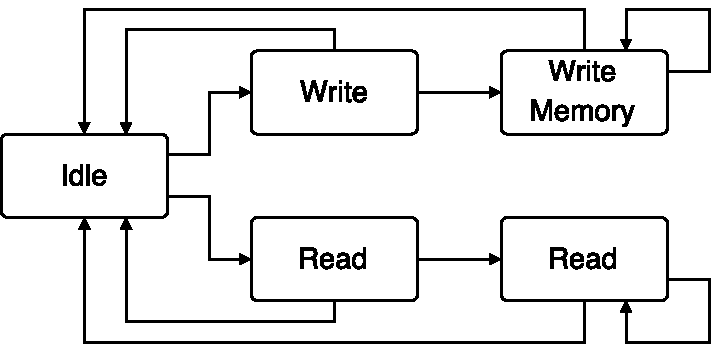
\includegraphics[width=0.5\linewidth]{fig/comm-fsm}
  \caption{State machine controlling the communication module.}
  \label{fig:comm-fsm}
\end{figure}

\figurename~\ref{fig:comm-fsm} shows the state machine controlling the operation
of the communication module. From the idle state, a transition to either the
Write or Read states can be triggered by asserting the PSEL signal on the APB
bus. Depending on wether or not the PWRITE signal is asserted, the state machine
will transition into the corresponding state. In this case, write refers to
writing data from the host to the receive buffer, and read refers to reading
data from the transmit buffer to the host. In the Write state, three bits in the
PADDR signal is used to further determine what is to happen. The possible
actions are as follows:

\begin{enumerate}
\item Write PWDATA to Receive Buffer. Transition to Idle state.
\item Set starting address register to PWDATA. Transition to Idle state.
\item Set end address register to PWDATA. Transition to Idle state.
\item Prepare to start transferring data from memory to Receive Buffer.
  Transition to Write Memory state.
\end{enumerate}

In the Write Memory state, read requests are generated on the MemPort bus and
received data is stored into the Receive Buffer. The Read and Read Memory states
have similar functionality, but writes data from the Transmit Buffer either
directly to the APB bus or to memory. In general, transfers of five 32-bit words
or less are done via the APB, while larger transfers go via memory. This is
however something that is specified in the SDK, not implemented in hardware.
That means that the system can be implemented to run on platforms without
on-board memory, as the MemPort interface can simply be tied off in that case.

The ConveyApbBridge-module serves, as the name implies, as a bridge between the
interfaces provided by the Convey PDK and the Communication module. The Dispatch
interface drives the APB bus, while the Memory Controller interface is wired
against the MemPort.


\clearpage


\section{Readout}

The Readout module extends the CARP platform with a reconfigurable Spiking
Neural Network operating in a data-driven fashion, synchronized to the clock of
state steps performed in the Cellular Automaton. Each layer of the network is
implemented as a stage in a pipeline. With every step of the CA, new input is
fed to the input layer and its output is fed as input to the next layer and so
on throughout the network. In other words, the number of state steps it takes
for data to propagate through the readout module as a whole is equal to the
number of layers in the network. The output from the final layer is routed back
into the CA. It is also stored in the Readout Buffer, from where it can be read
back to the host.

\begin{figure}[ht]
  \centering
  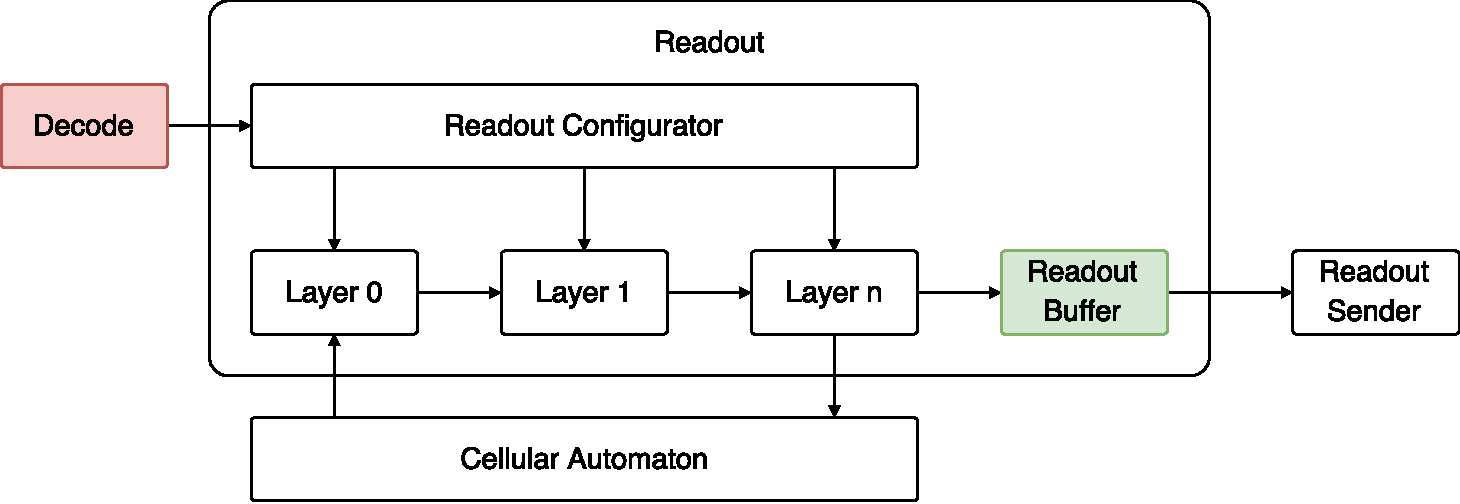
\includegraphics[width=\linewidth]{fig/readout-io}
  \caption{Logical overview of the Readout module.}
  \label{fig:readout-io}
\end{figure}

\figurename~\ref{fig:readout-io} shows, at a high level of abstraction, how the
Readout module is connected to the CARP system as whole. A subset of cell states
are routed out of the CA and into the Readout module as input to the first layer
of the network, the input layer. Within each layer, a number of neurons process
the input to the layer, as shown in \figurename~\ref{fig:readout-layer}. Based
on this input, they update their activation values, which again are fed to the
next layer to be used as input to those neurons in the next step.

\begin{figure}[ht]
  \centering
  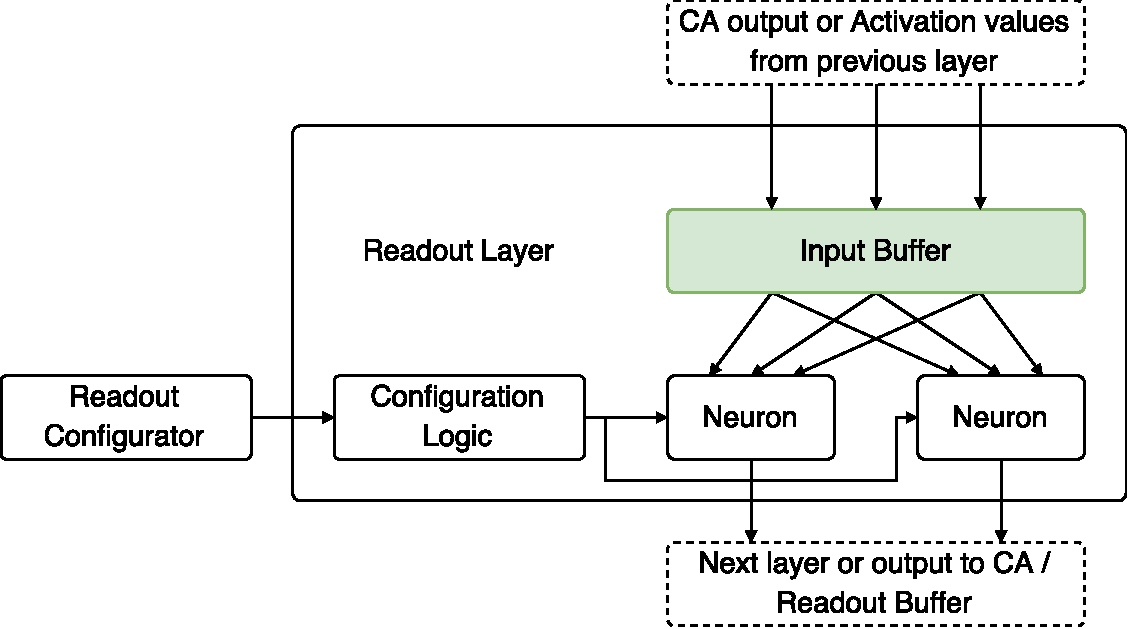
\includegraphics[width=0.8\linewidth]{fig/readout-layer}
  \caption{Logical overiew of one network layer in the Readout module.}
  \label{fig:readout-layer}
\end{figure}

The activation value of a neuron can be either 0 or 1, based on a very simple
calculation, as shown in \figurename~\ref{fig:readout-neuron}. For each of its
incoming edges, a neuron has a pair of registers, the edge weight and a counter.
The counter keeps track of how many spikes the neuron has received via the
corresponding edge, and the weight is a threshold, indicating how many spikes
must arrive via the edge before the neuron can fire. When all counters values
are equal to or greater than their weights, the neuron fires and the counters
are reset.

\begin{figure}[ht]
  \centering
  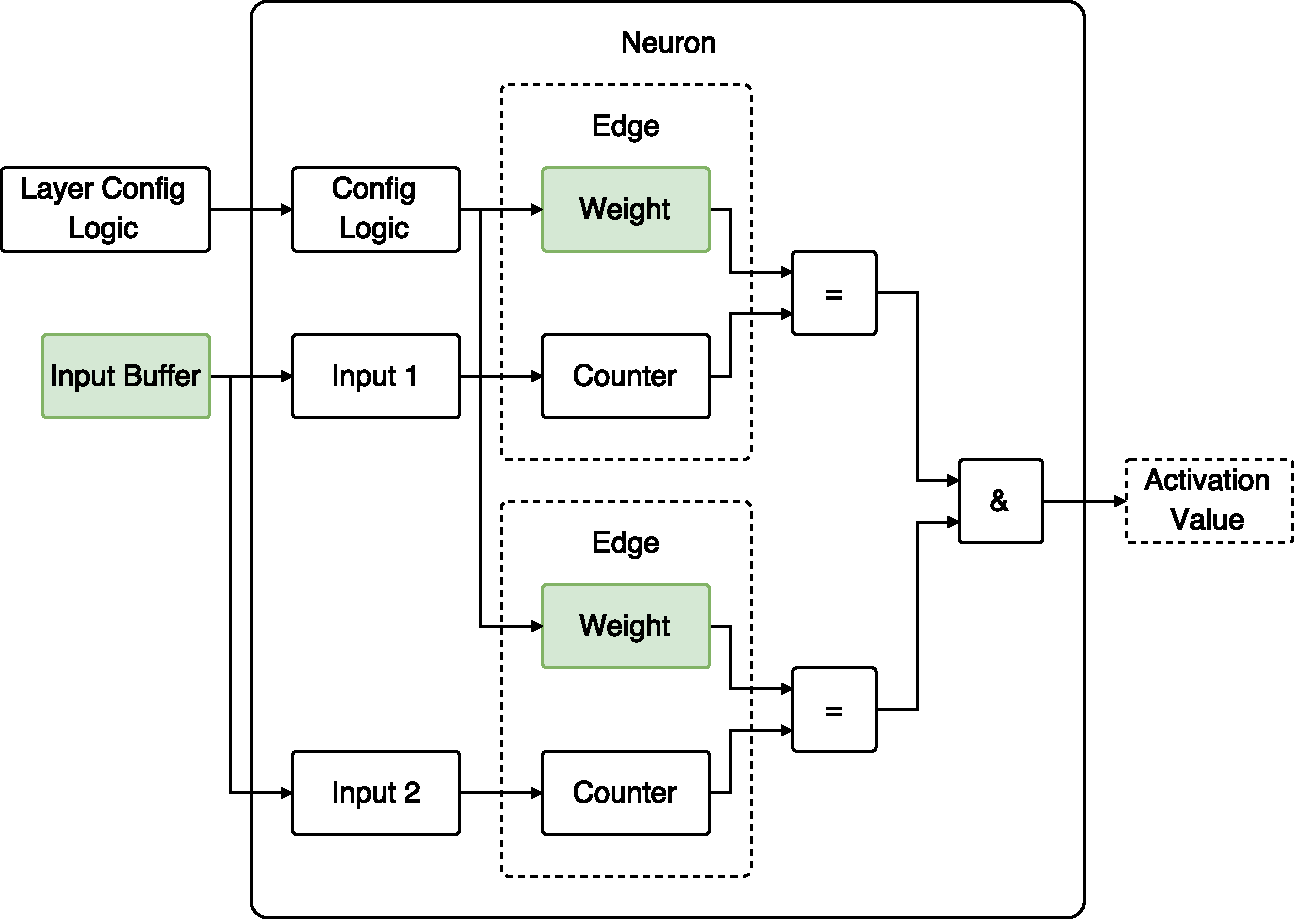
\includegraphics[width=0.8\linewidth]{fig/readout-neuron}
  \caption{Logical overview of a single neuron in the Readout module.}
  \label{fig:readout-neuron}
\end{figure}

To reduce the amount of resources required for the implementation, some
restrictions apply with regards to which network topologies are possible to
implement. All networks must be entirely feed-forward, that is they can not
contain any recurrent connections, and the final layer must contain only a
single neuron. The topology of a network is given as a parameter to the module
at synthesis time, and can not be reconfigured while the system is running. It
describes how many layers the network consists of and how many neurons each of
them consist of. Networks are also implemented fully connected, all neurons in a
layer are connected to all neurons in the previous layer.


The module can be in one of two states, the default Processing state and the
Configuration state. In the Processing state, data flows through the network in
the manner described above. 



\clearpage

\section{Cellular Automata}

\section{Parameterization}

\section{Software API}

\cleardoublepage
%%% Local Variables:
%%% mode: latex
%%% TeX-master: "../thesis"
%%% End:
